\documentclass[11pt,a4paper]{article}

\usepackage[margin=2.3cm]{geometry}

\usepackage{graphicx}

\usepackage{xcolor}

\usepackage{booktabs}

\usepackage{longtable}

\usepackage{array}

\usepackage{hyperref}

\usepackage{fancyvrb}

\usepackage{caption}

\usepackage{float}

\usepackage{setspace}

\setstretch{1.08}

\hypersetup{colorlinks=true, linkcolor=blue, urlcolor=blue}

\begin{document}

\begin{titlepage}

\centering


\includegraphics[width=0.34\textwidth]{assets/university_of_sheffield_logo.jpg}\\[1.4cm]

{\LARGE COM6523 Software Reengineering\\[0.2cm]Group Project Report\par}

\vspace{1cm}

{\large Group PG\_05\par}

\vfill

\end{titlepage}

\tableofcontents

\newpage

\begin{longtable}{p{0.43\textwidth} p{0.43\textwidth}}
\toprule
Item & Details \\
\midrule
Group ID & PG\_05 \\
\addlinespace
Group Repository & https://github.com/TUOS-COM-Reengineering-2026/group-project-pg\_05 \\
\addlinespace
Selected Open-Source System & aio-libs/yarl \\
\addlinespace
Original Repository & https://github.com/aio-libs/yarl \\
\addlinespace
Snapshot Commit Used & e25e8d23e6912db52a23513ef1f6a17f889751ef \\
\addlinespace
Main Reengineering Target & URL path-resolution responsibilities: URL.join(), URL.\_make\_child(), URL.joinpath(), and the / operator \\
\addlinespace
\bottomrule
\end{longtable}


\begin{longtable}{p{0.43\textwidth} p{0.43\textwidth}}
\toprule
Member & Main Responsibilities \\
\midrule
Dibing Bai & Project setup, repository preparation, baseline environment evidence, and focused local regression testing. \\
\addlinespace
Yongjiang Liu & Project coordination, coursework requirement interpretation, target selection, system understanding, GitHub branch and PR integration, and final report/evidence synthesis. \\
\addlinespace
Jingxuan Wang & Static analysis, Radon and code-smell interpretation, restructuring rationale, and requirement-alignment review. \\
\addlinespace
Ziqi Zhao & Regression test design for URL.join(), URL.joinpath(), and the / operator; URL.join() refactoring evidence; and before/after evaluation. \\
\addlinespace
Xuhao Zhou & Upstream evolution analysis, dynamic analysis evidence, GitHub workflow/local verification evidence, and document preparation. \\
\addlinespace
\bottomrule
\end{longtable}


\section*{Introduction}
\addcontentsline{toc}{section}{Introduction}


This project reengineers aio-libs/yarl, a Python library that provides a structured URL object for parsing, constructing, normalising, quoting, and transforming URLs. The library is widely relevant because URL manipulation sits underneath HTTP clients, web frameworks, asynchronous networking tools, and data-processing code that handles links. Instead of forcing users to splice URL strings manually, yarl exposes a central URL class with methods for inspecting components, changing paths, manipulating queries, and resolving relative URLs.


yarl was selected because it satisfies the coursework requirements for a meaningful reengineering subject. It is an active open-source system, it has a substantial Git history, it includes runnable tests, and it contains enough internal complexity to support repository mining, static analysis, dynamic analysis, regression testing, and controlled restructuring. The group repository was seeded from upstream snapshot e25e8d23e6912db52a23513ef1f6a17f889751ef before any reengineering work began, so all analysis and changes are anchored to a fixed baseline.


The aim was not to redesign yarl's public API or add user-facing features. Because URL is the main public abstraction, compatibility is more important than novelty. The project therefore focused on conservative internal restructuring around URL path resolution. Static analysis identified yarl/\_url.py as the central and most overloaded module, with URL.join() and URL.\_make\_child() both rated C (17) by Radon at baseline. These methods are connected to public behaviours through URL.join(), URL.joinpath(), and the / operator, but their detailed path-selection and path-assembly responsibilities could be decomposed without changing the external interface.


The completed work added focused regression tests, extracted URL.join() path/query/fragment logic into helper functions, moved join-specific helpers into yarl/\_join.py, moved child path assembly from URL.\_make\_child() into yarl/\_path.py, added dynamic analysis evidence, restored a minimal regression workflow, and refreshed final local verification evidence. The final local pytest run reported 1129 passed, 103 skipped, and 2 xfailed, while the key complexity results improved from URL.join C (17) to B (8) and URL.\_make\_child C (17) to A (1).


\section*{Understanding the System}
\addcontentsline{toc}{section}{Understanding the System}


\subsection*{System Purpose and Architecture}


At a high level, yarl is intentionally compact from a user's point of view. Most interactions pass through the URL class: callers construct a URL, inspect its parts, update selected components, join relative references, or append child path segments. Internally, however, this apparently simple interface must handle encoded and decoded forms, absolute and relative URLs, authority components, query strings, fragments, path normalisation, and quoting rules. This creates a natural tension between a convenient public facade and a large amount of internal URL semantics.


The original system is a URL manipulation library rather than an end-user application. Its main function is to turn URL strings into structured URL objects, then allow callers to inspect or change components such as scheme, host, path, query, and fragment. It also has to preserve difficult URL details such as percent-encoded characters, host encoding, relative references, and path normalisation. This is why the public API looks simple while the internal implementation has to coordinate several specialised concerns.


The architecture reflects that tension. Users mostly interact with URL in yarl/\_url.py, but the implementation also depends on parsing, quoting, query, path, and cache helpers. This means \_url.py is both the stable public facade and the place where many helper responsibilities meet. The report therefore treats \_url.py as an architectural coordination point rather than merely as a large file. The reengineering problem was to reduce detailed responsibility inside that coordinator without changing the behaviour users depend on.


\begin{longtable}{p{0.29\textwidth} p{0.29\textwidth} p{0.29\textwidth}}
\toprule
Module & Responsibility & Reengineering relevance \\
\midrule
yarl/\_url.py & Defines URL and most public URL transformation methods. & Central coordinating module; baseline hotspot for complexity and responsibility concentration. \\
\addlinespace
yarl/\_parse.py & Splits and reassembles URL components. & Important dependency for URL construction and dynamic traces. \\
\addlinespace
yarl/\_path.py & Normalises path segments and now assembles child paths. & Appropriate home for path-specific helper logic moved out of \_url.py. \\
\addlinespace
yarl/\_query.py & Builds and updates query-string data. & Supports URL.update\_query() and query-related public API behaviour. \\
\addlinespace
yarl/\_quoting\_py.py / \_quoting\_c.pyx & Quote and unquote URL components in Python or accelerated Cython form. & Runtime traces show quoting remains a frequent low-level operation. \\
\addlinespace
yarl/\_join.py & Private module introduced for URL.join() helper decisions. & System-level restructuring result that localises join-specific logic. \\
\addlinespace
\bottomrule
\end{longtable}


This structure shows why \_url.py was the natural place to inspect first. The module is not merely large; it coordinates many different URL behaviours. A change inside it can affect public behaviour, so any reengineering target inside URL needs a strong regression safety net and careful before/after evaluation.


The evolution evidence shows that this architecture has changed over time. The LOC sample in Submission/analysis/loc\_over\_time.csv records growth from v0.0.1 with 2 files, 380 source lines, and 825 test lines to the analysed HEAD snapshot with 24 files, 2764 source lines, and 6407 test lines. The test suite grew faster than the production code, which suggests that maintainers increasingly protected compatibility as the library matured. This influenced our own approach: any restructuring needed to be test-led rather than speculative.


The file-count growth also shows architectural decomposition. Early versions were smaller and more concentrated. Later versions split responsibilities into modules such as \_parse.py, \_path.py, \_query.py, and the quoting implementations. Several 2024 upstream commits explicitly moved URL parsing, query-string functions, quoters, and path functions into their own modules. Our restructuring follows this direction by continuing to move path-resolution details away from \_url.py and into focused private modules.


\subsection*{Evolution and Original Reengineering Evidence}


The upstream repository contained 1927 commits at the analysed snapshot, which made it suitable for version repository analysis. The group mined commit activity, LOC over time, and refactoring-related commit messages into Submission/analysis. The LOC evidence shows growth from a small utility into a mature library with a larger test suite than source-code base, which supports the strategy of using automated tests as the primary guard against behavioural regression.


The driving forces behind the system's changes appear to be compatibility, packaging, performance, and maintainability rather than feature expansion alone. The refactoring-commit search found many maintenance commits in 2024, including removal of internal SplitResult usage, cleanup of \_url.py constants, movement of parsing/query/path functions into separate modules, and small cleanups around URL.join() and child-path creation. These commits indicate a mature project where internal structure is regularly adjusted to preserve a clean implementation behind a stable API.


The size and complexity trend also explains why a conservative target was chosen. A library with more than 1900 upstream commits and over 9000 sampled source-plus-test lines is not a safe place for broad redesign in a short coursework project. The evidence instead suggested a smaller intervention: identify a central responsibility that had become complex, add focused tests, move the responsibility to an existing helper area, and then compare the result using the same analysis tools.


\begin{figure}[H]\centering

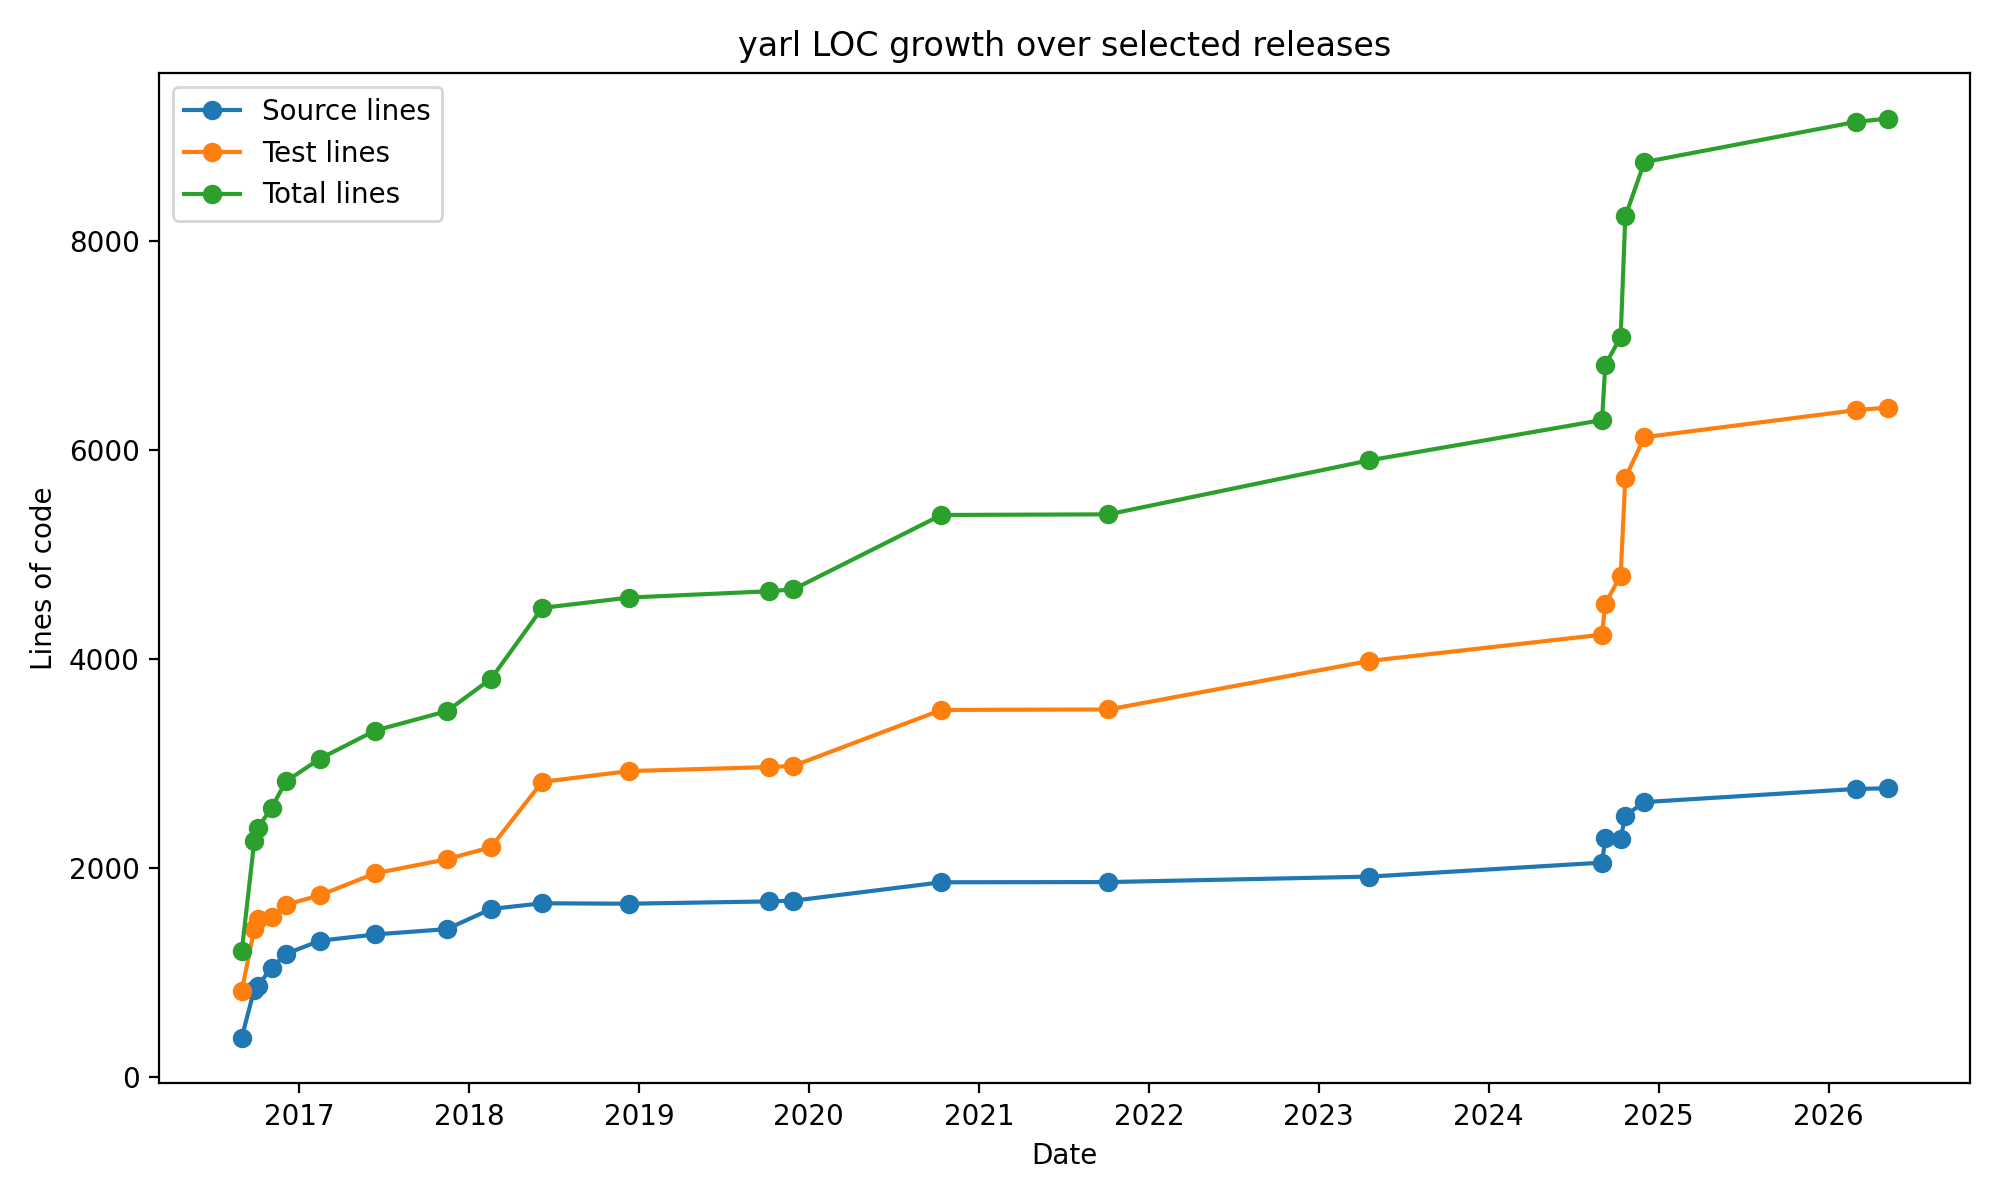
\includegraphics[width=0.82\textwidth]{assets/report_image_2.png}

\end{figure}

\begin{center}\small Figure 1. LOC growth over selected yarl revisions.\end{center}

\begin{figure}[H]\centering

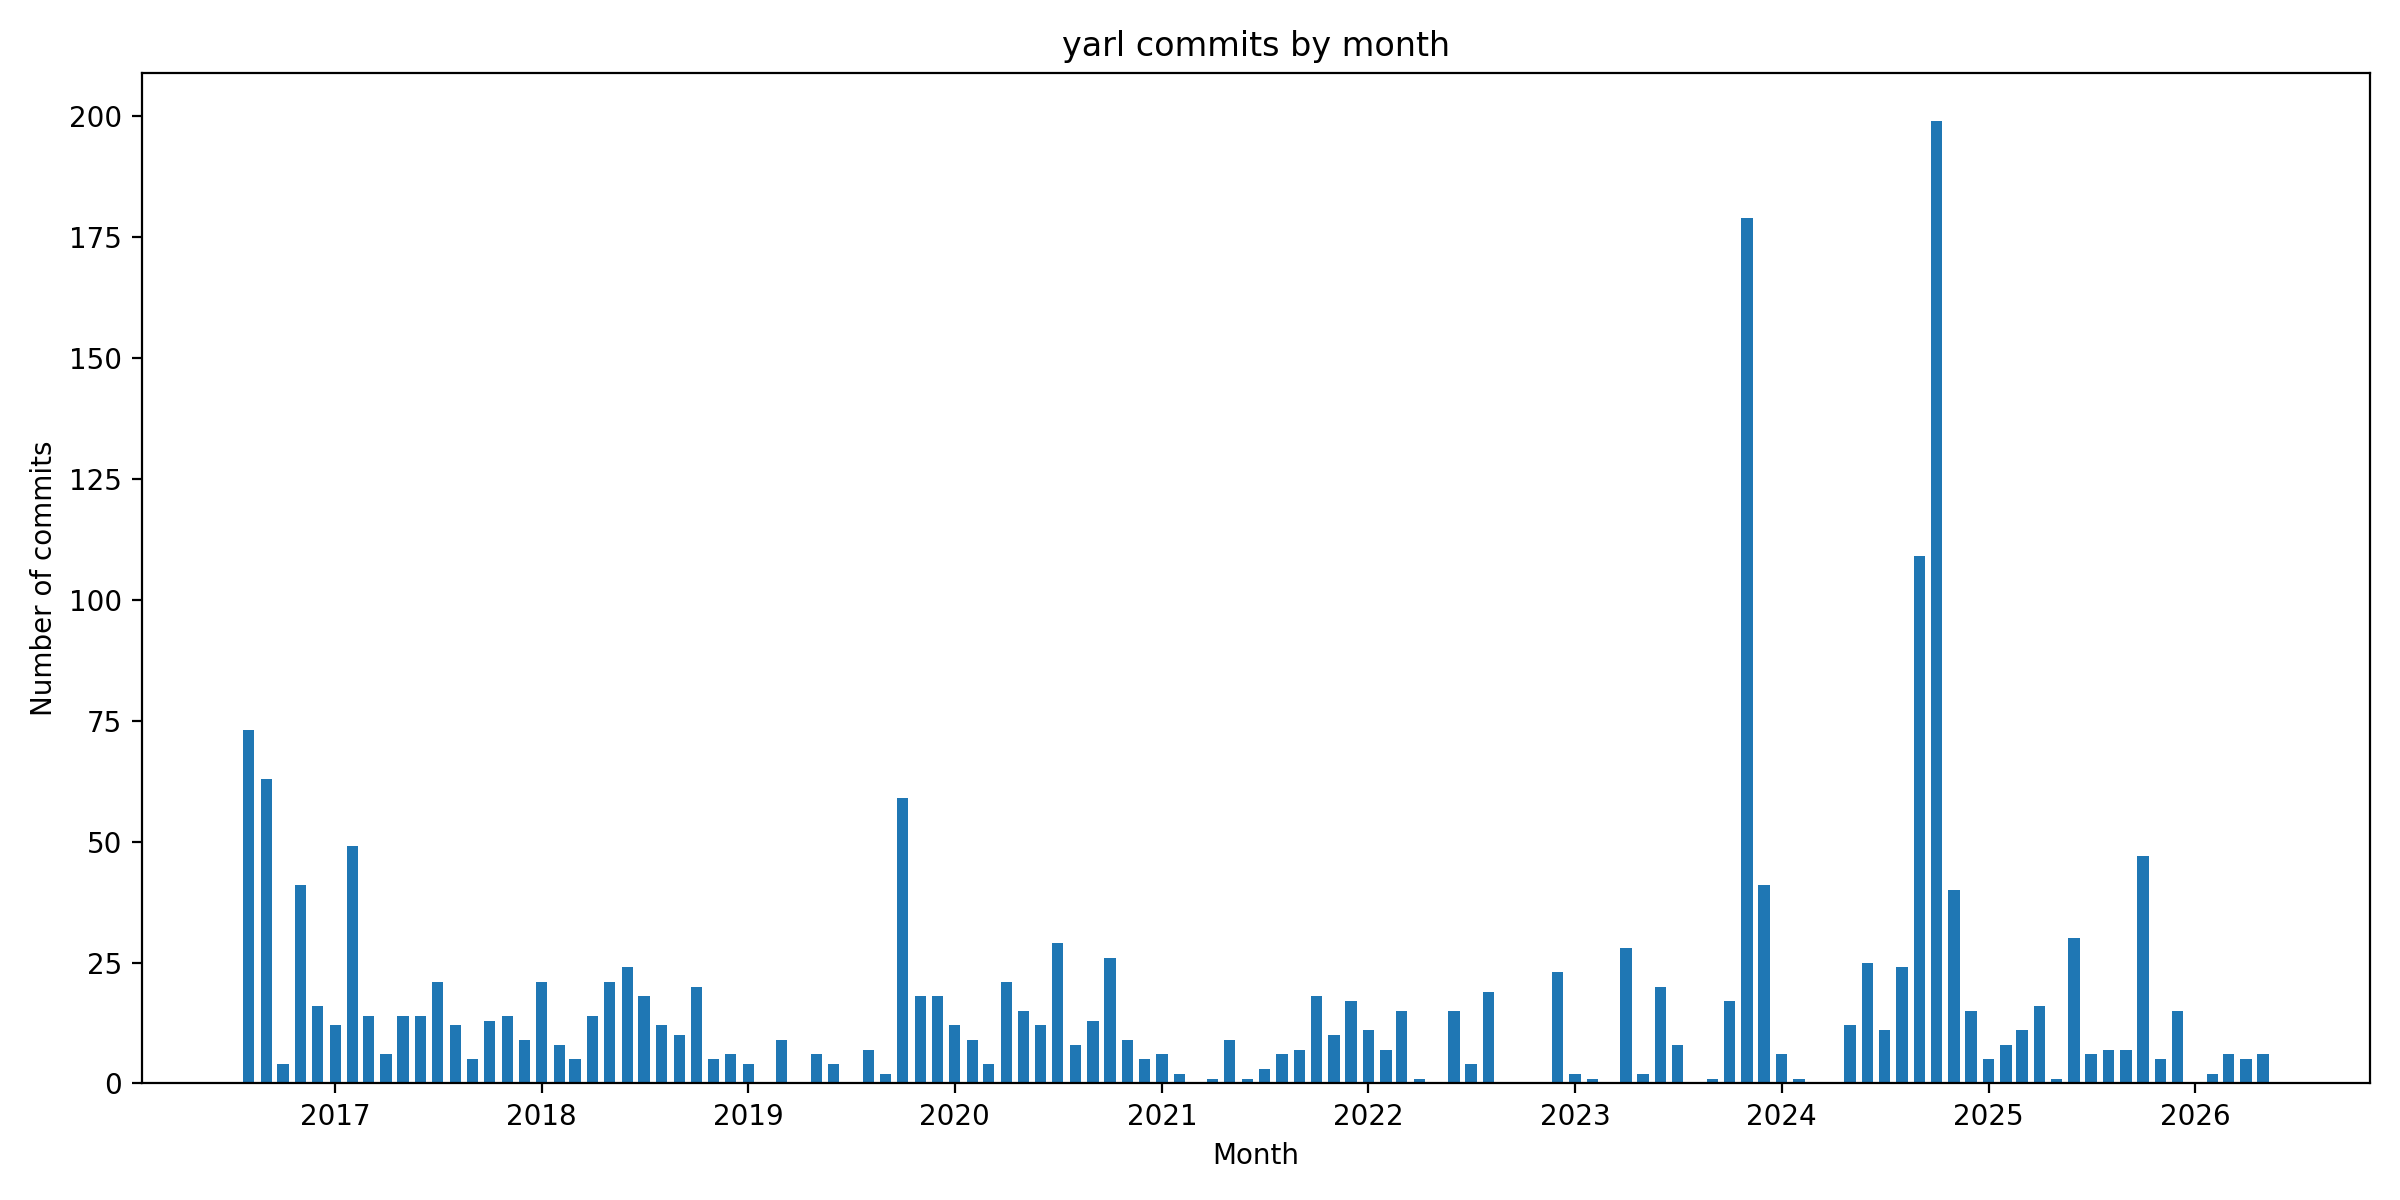
\includegraphics[width=0.82\textwidth]{assets/report_image_3.png}

\end{figure}

\begin{center}\small Figure 2. Upstream commit activity by month.\end{center}

The original developers had already performed maintenance and cleanup work in the same area. The refactoring commit search found URL.join-related commits including 'Refactor URL.join to avoid intermediate dict' and 'Small cleanups to URL.join'. This does not prove that URL.join() was defective, but it does show that the upstream maintainers had previously found the method worth simplifying. Our approach therefore followed the style of the original project: preserve public behaviour and improve internal structure incrementally.


The original developers' reengineering efforts were partly successful because they created the structure that made our narrower restructuring possible. For example, moving path functions into yarl/\_path.py made it reasonable for our project to move child path assembly there as well. The later URL.join cleanup commits also showed that maintainers had already considered join logic worth simplifying. However, the base snapshot still left URL.join() and URL.\_make\_child() with C (17) Radon complexity scores, so the earlier work had not removed all path-resolution complexity from \_url.py.


This conclusion matters for target selection. We did not choose URL.join() simply because an upstream commit name mentioned it. We chose it because repository history, module architecture, static complexity, and regression-test feasibility all pointed in the same direction. URL.\_make\_child() was then selected as a related second target because it supports URL.joinpath() and the / operator and because its path assembly responsibility naturally belonged with the path helpers.


\subsection*{Static Analysis, Code Smells, and Test Adequacy}


Baseline Radon complexity results identified several non-trivial methods in yarl/\_url.py. URL.build() had the highest complexity at E (38), but it handles a broad construction interface with many public behaviours, so it was judged too risky for the project timeframe. A more focused and still meaningful opportunity existed in URL.join() and URL.\_make\_child(), both rated C (17). These methods sit behind path-resolution behaviours that can be covered with targeted regression tests.


The remaining code smells in the base snapshot were therefore responsibility concentration and method complexity. URL.build() had a higher complexity score, but it also had a broader construction role and many optional inputs. Refactoring it would risk changing validation or construction semantics across a larger part of the API. URL.join() and URL.\_make\_child() were better targets because their complexity was significant, their behaviours could be expressed through focused public-API tests, and their responsibilities matched existing helper modules.


The impact of these smells is practical rather than cosmetic. URL resolution contains many edge cases: absolute URL replacement, network-path references, empty paths, root-relative paths, current-directory relative paths, query-only and fragment-only references, dot-segment handling, and encoded path values. When these rules sit inside a public coordinating method, a future maintainer has to understand several concerns at once. Moving the details into named helpers reduces the review burden and makes future changes less likely to disturb unrelated URL behaviour.


\begin{longtable}{p{0.29\textwidth} p{0.29\textwidth} p{0.29\textwidth}}
\toprule
Evidence type & Observation & How it influenced the strategy \\
\midrule
Repository history & URL.join() had prior upstream cleanup/refactoring commits. & Selected a maintenance area already recognised by original developers. \\
\addlinespace
Static analysis & URL.join() and URL.\_make\_child() were both C (17); \_url.py was the central module. & Targeted path-resolution responsibility rather than a broad rewrite. \\
\addlinespace
Existing tests & Baseline pytest passed with 1115 passed, 103 skipped, 2 xfailed. & Existing tests gave a general safety net before adding focused cases. \\
\addlinespace
Focused tests & New tests were added for URL.join(), URL.joinpath(), and the / operator. & Protected the exact behaviours affected by the restructuring. \\
\addlinespace
Dynamic analysis & Final traces showed URL.join delegating to yarl.\_join and URL.joinpath delegating through \_make\_child to yarl.\_path. & Confirmed that the new private helpers are exercised in representative runtime scenarios. \\
\addlinespace
\bottomrule
\end{longtable}


The main smell was responsibility concentration rather than a visible user-facing bug. \_url.py acted as the public facade and also contained detailed path-resolution rules. The reengineering strategy therefore aimed to reduce method-level complexity and module responsibility while keeping URL as the public entry point.


The existing tests were strong enough to give broad confidence in the library, but they were not sufficient as the only regression strategy for this project. The baseline suite showed that the cloned snapshot could run, but the coursework changes touched specific path-resolution behaviours. The group therefore added tests/test\_url\_join\_regression.py and tests/test\_url\_joinpath\_regression.py to cover the behaviours most likely to be affected. This directly answers the brief's question about whether existing test cases were enough: they were a useful base, but targeted reengineering required additional focused tests.


Using multiple advanced techniques made the understanding more reliable. Repository mining explained how the system had evolved and what maintainers had previously restructured. Static analysis identified the current hotspots and code smells. Manual architecture inspection explained why those hotspots mattered. Dynamic analysis later confirmed that the new helper paths were actually exercised at runtime. Regression testing then protected behaviour. The target was therefore selected through connected evidence rather than by relying on one metric in isolation.


The significance of the remaining smells was therefore judged by their likely maintenance impact. A complex method in a rarely used internal script would be less important than a complex method in the central URL class. URL.join() and URL.\_make\_child() matter because they sit behind everyday URL path operations and because mistakes in URL resolution can be subtle: a method may return a syntactically valid URL while still preserving the wrong query, fragment, encoded segment, or base path. This is why the analysis connected code smells to behavioural risk before choosing the final restructuring target.


This is also why the group kept the selected scope close to path-resolution responsibility. The analysis did not justify removing functionality or changing URL semantics; it justified making existing behaviour easier to understand, test, and maintain.


\section*{Restructuring the System}
\addcontentsline{toc}{section}{Restructuring the System}


\subsection*{Restructuring Requirements}


The desired outcome was improved maintainability and modularity, not new functionality. The public API had to remain stable: URL, URL.join(), URL.joinpath(), and the / operator should still be called in the same way and return the same results for the protected cases. The internal goal was to make path-resolution responsibilities easier to locate by moving join-specific logic into yarl/\_join.py and child path assembly into yarl/\_path.py. This directly addressed the overloaded role of yarl/\_url.py identified during system understanding.


There were also compromises between quality attributes. A deeper rewrite might have produced a more radical design, but it would also increase compatibility risk and require broader testing. A performance-oriented change might have introduced caching or lower-level optimisations, but the project evidence did not show performance as the main problem. The achievable requirement within the timeframe was therefore a conservative structural improvement: reduce complexity in the central URL methods, preserve behaviour, and keep moved helpers private so the public maintenance contract did not grow.


The implementation strategy followed the brief's expectation for both system-level restructuring and unit-level refactoring. At the unit level, complex methods were simplified by extracting named helper decisions. At the system level, those helper decisions were placed into modules with clearer responsibility boundaries. Work was split into small commits so tests and evidence could be checked after each step. This also kept the reengineering feasible for a group project rather than turning it into a complete redesign of yarl.


\begin{longtable}{p{0.29\textwidth} p{0.29\textwidth} p{0.29\textwidth}}
\toprule
ID & Requirement & Rationale \\
\midrule
R1 & Preserve the public API and existing behaviour. & URL, URL.join(), URL.joinpath(), and the / operator are relied on by users. \\
\addlinespace
R2 & Add focused regression tests before relying on refactoring. & URL path resolution has edge cases around relative paths, encoded segments, queries, and fragments. \\
\addlinespace
R3 & Reduce method complexity in URL.join() and URL.\_make\_child(). & Both were C (17) in the baseline Radon report. \\
\addlinespace
R4 & Move path-specific responsibilities out of yarl/\_url.py where appropriate. & \_url.py should coordinate URL objects, not own all detailed path-assembly rules. \\
\addlinespace
R5 & Make verification repeatable locally and visible in the repository. & Remote CI was constrained by the GitHub organisation account, so committed local evidence was essential. \\
\addlinespace
\bottomrule
\end{longtable}


\subsection*{Regression Tests Before Refactoring}


The first code change added tests/test\_url\_join\_regression.py. These tests cover relative path resolution, current-directory paths, root-relative paths, query-only references, fragment-only references, network-path references, and absolute URL replacement. The second test file, tests/test\_url\_joinpath\_regression.py, covers multi-segment child path assembly, query and fragment cleanup when appending children, dot-segment handling, relative URL behaviour, encoded path segment preservation, and the / operator.


The second focused test file, tests/test\_url\_joinpath\_regression.py, protected the child-path restructuring. It covered multi-segment child path assembly, query and fragment cleanup, dot-segment handling for absolute URLs, current relative-URL behaviour, encoded path segment preservation, and the / operator. These were chosen because they are public behaviours that reach URL.\_make\_child() even though the method itself is private.


This test design was deliberately behaviour-first. The group did not write tests that assert private helper names or internal call order, because that would make the tests brittle and reduce future maintainability. Instead, the tests describe what users should observe before and after the restructuring. The final full test suite then provided a broader safety net, while the focused tests explained exactly why the selected reengineering area was protected.


The test order matters. The focused tests were added before relying on the internal restructuring so that expected behaviours were documented as executable checks. The final local focused checks showed 7 passed for URL.join regression tests, 7 passed for URL.joinpath regression tests, and 143 passed for existing URL join/joinpath/div tests from tests/test\_url.py.


\subsection*{Unit-Level Refactoring: URL.join()}


URL.join() originally mixed several decisions in one public method: input type checking, scheme selection, authority replacement, relative-path resolution, query selection, and fragment selection. The refactoring kept the public method in URL but extracted component-specific decisions into private helpers. The method now coordinates URL state and delegates path, query, and fragment decisions to \_resolve\_join\_path(), \_resolve\_join\_query(), and \_resolve\_join\_fragment().


After helper extraction, the helper functions were moved into yarl/\_join.py. This was the system-level part of the same change: join-specific logic no longer made \_url.py larger, and future maintainers can inspect join behaviour in a focused private module. URL.join() remained the public entry point and still returns URL objects through the existing from\_parts flow.


This change answered the maintainability requirement by separating decisions that had previously been interleaved in one public method. URL.join() still owns the public operation and final URL construction, but \_resolve\_join\_path(), \_resolve\_join\_query(), and \_resolve\_join\_fragment() describe the internal decisions separately. That makes the code easier to review because a maintainer can inspect path, query, or fragment behaviour without reading the whole join method as one block.


The helper module remains private, which avoids a conflict between extensibility and compatibility. It improves internal extensibility for maintainers by creating a focused place for join behaviour, but it does not expose a new supported API that users could depend on. This is important for a library such as yarl, where adding public surface area can create future maintenance cost.


\subsection*{System-Level Restructuring: Child Path Assembly}


The second reengineering task targeted URL.\_make\_child(), the private method behind URL.joinpath() and URL.\_\_truediv\_\_(). Baseline analysis rated URL.\_make\_child as C (17), and the method contained path-specific assembly logic that was better aligned with yarl/\_path.py. The refactoring moved this responsibility into \_make\_child\_path() and smaller helper functions in \_path.py, while URL.\_make\_child() now coordinates the URL state and calls from\_parts().


This extended the same restructuring narrative as the URL.join() work. yarl/\_url.py remains the public facade and coordinator, while path-resolution details are progressively delegated to path-focused private modules. The public API did not change: users still call URL.joinpath() or use the / operator in the same way.


The \_make\_child() change addressed a module-level overload. Before the change, yarl/\_url.py did not only coordinate URL object state; it also assembled child path segments for joinpath() and the / operator. After the change, URL.\_make\_child() delegates path calculation to \_make\_child\_path() in yarl/\_path.py and then uses the existing URL construction pathway. This keeps \_url.py focused on object coordination and moves path-specific rules into the path module.


The complexity outcome shows the effect of this decision. URL.\_make\_child() moved from C (17) to A (1), while \_make\_child\_path() remained B (8) and its smaller helpers stayed A-rated. This is not just a numerical improvement. It means the unavoidable path-assembly branches are now grouped with path helpers, while the public URL class method reads as a short coordination step. That is the quality improvement the restructuring requirement asked for.


\subsection*{Dynamic Analysis}


To satisfy the COM6523 expectation for advanced techniques beyond static metrics, the group added a dynamic analysis script in Submission/analysis/collect\_dynamic\_metrics.py. It traces representative scenarios for URL.join(), URL.joinpath(), URL.build(), and URL.update\_query(), then writes call-count and module-edge CSV files plus a markdown summary.


\begin{longtable}{p{0.29\textwidth} p{0.29\textwidth} p{0.29\textwidth}}
\toprule
Scenario & Runtime evidence & Interpretation \\
\midrule
URL.join & Trace includes URL.join -> yarl.\_join.\_resolve\_join\_path / \_resolve\_join\_query / \_resolve\_join\_fragment. & The final public method delegates to the new private join module. \\
\addlinespace
URL.joinpath & Trace includes URL.joinpath -> URL.\_make\_child -> yarl.\_path.\_make\_child\_path. & The child-path restructuring is exercised at runtime. \\
\addlinespace
URL.build & Trace includes URL.build, query helpers, host encoding, and path normalisation. & High complexity exists elsewhere, but this broad method was intentionally not refactored. \\
\addlinespace
URL.update\_query & Trace includes query parsing and quoting helpers. & Shows the wider URL module remains a coordinator for multiple URL behaviours. \\
\addlinespace
\bottomrule
\end{longtable}


The dynamic evidence supports the core argument rather than replacing static analysis. Static analysis identified where complexity was concentrated; dynamic analysis showed that the new helper modules are part of real execution paths in the final repository.


The dynamic evidence also helped compare behaviour before and after in a way that static metrics cannot. The final trace scenarios exercised URL.join(), URL.joinpath(), URL.build(), and URL.update\_query(). The joinpath trace recorded calls into yarl.\_path:\_make\_child\_path and \_extend\_with\_child\_segments, while the join scenario still exercised the URL construction and quoting pathway. This confirmed that the moved helper code was part of representative runtime behaviour in the final repository.


\subsection*{Evaluation}


\begin{longtable}{p{0.21\textwidth} p{0.21\textwidth} p{0.21\textwidth} p{0.21\textwidth}}
\toprule
Measure & Before & After & Interpretation \\
\midrule
Full local pytest & 1115 passed, 103 skipped, 2 xfailed & 1129 passed, 103 skipped, 2 xfailed & The increase reflects added regression tests; no full-suite regression was introduced. \\
\addlinespace
URL.join complexity & C (17) & B (8) & The public method became shorter and easier to reason about. \\
\addlinespace
URL.\_make\_child complexity & C (17) & A (1) & Path assembly moved out of the coordinating URL method. \\
\addlinespace
\_resolve\_join\_path & Not extracted & B (6) & Join path logic is isolated in a private helper. \\
\addlinespace
\_make\_child\_path & Not extracted & B (8) & Child path logic is isolated in yarl/\_path.py. \\
\addlinespace
Focused local checks & Not present at baseline & 7 URL.join tests, 7 URL.joinpath tests, 143 existing join/joinpath/div tests passed & Targeted regression evidence now directly covers changed behaviours. \\
\addlinespace
\bottomrule
\end{longtable}


A minimal GitHub Actions workflow was restored with workflow\_dispatch, push, and pull\_request triggers for URL-related code and tests. A real remote run was checked, but GitHub reported that the job was not started because recent account payments had failed or the spending limit needed to be increased. No runner was allocated, so the failure was an account/billing limitation rather than a project test failure. The final local verification evidence was therefore committed under Submission/final-check as the authoritative validation record.


The main comparison method was regression testing. Focused tests checked the behaviours most directly connected to the changed code, existing URL join/joinpath/div tests checked nearby behaviour, and the full local suite checked the wider library. The final recorded result was 1129 passed, 103 skipped, and 2 xfailed, with 7 focused URL.join tests, 7 focused URL.joinpath tests, and 143 existing URL join/joinpath/div tests passing. This provides stronger evidence than only saying that the code still imports.


The structural comparison used Radon and the local evidence script. URL.join() improved from C (17) to B (8), URL.\_make\_child() improved from C (17) to A (1), and the new helpers stayed within acceptable A/B complexity ranges. This directly demonstrates the impact of the changes on maintainability. The GitHub Actions billing limitation prevented a successful remote runner allocation, but tools/run\_local\_checks.py made the same final checks repeatable and saved their outputs under Submission/final-check.


\begin{figure}[H]\centering

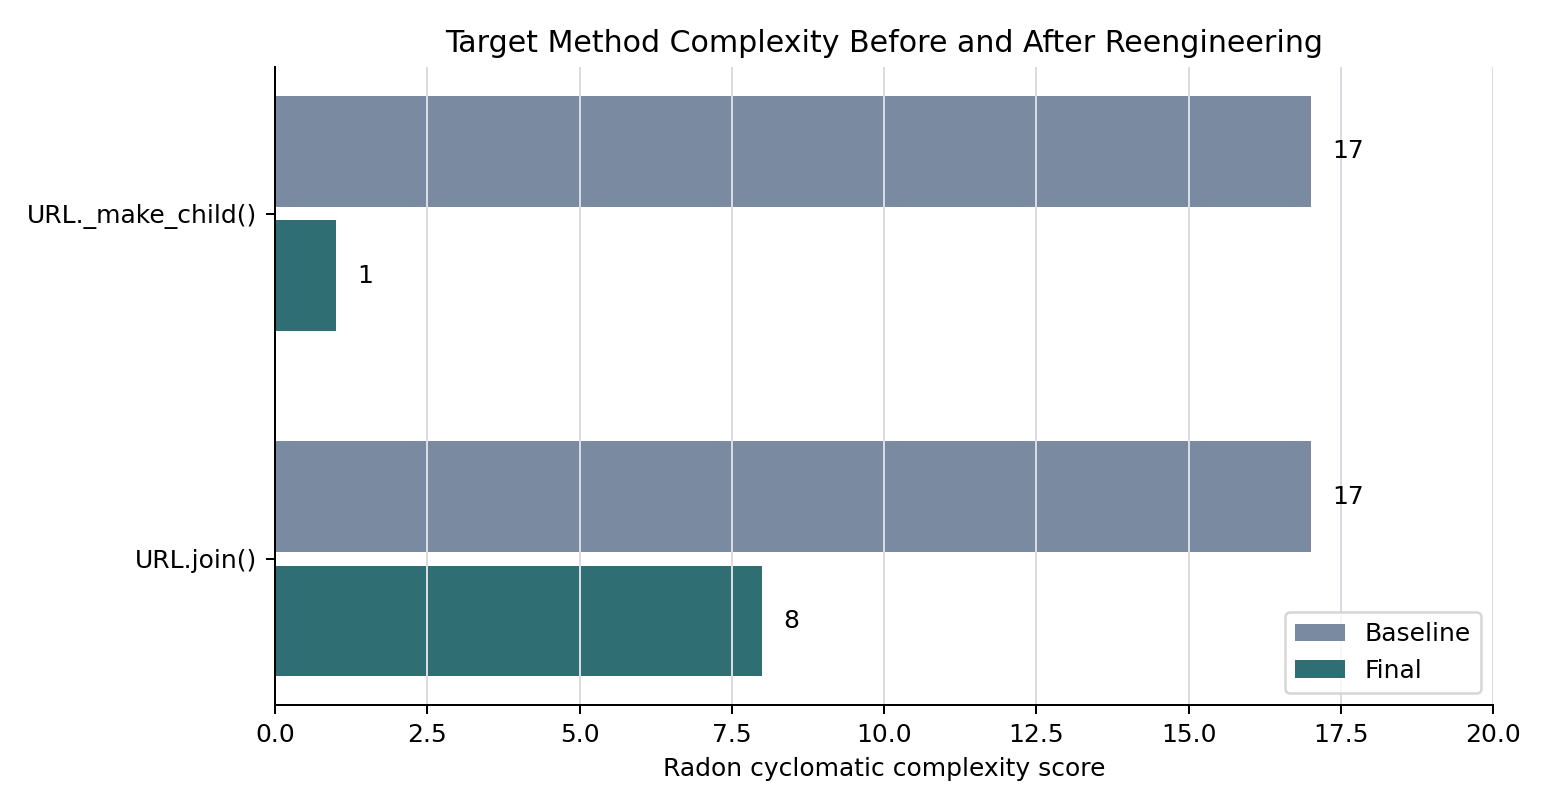
\includegraphics[width=0.82\textwidth]{assets/report_image_4.png}

\end{figure}

\begin{center}\small Figure 3. Radon complexity for the two target methods before and after reengineering.\end{center}

\begin{figure}[H]\centering

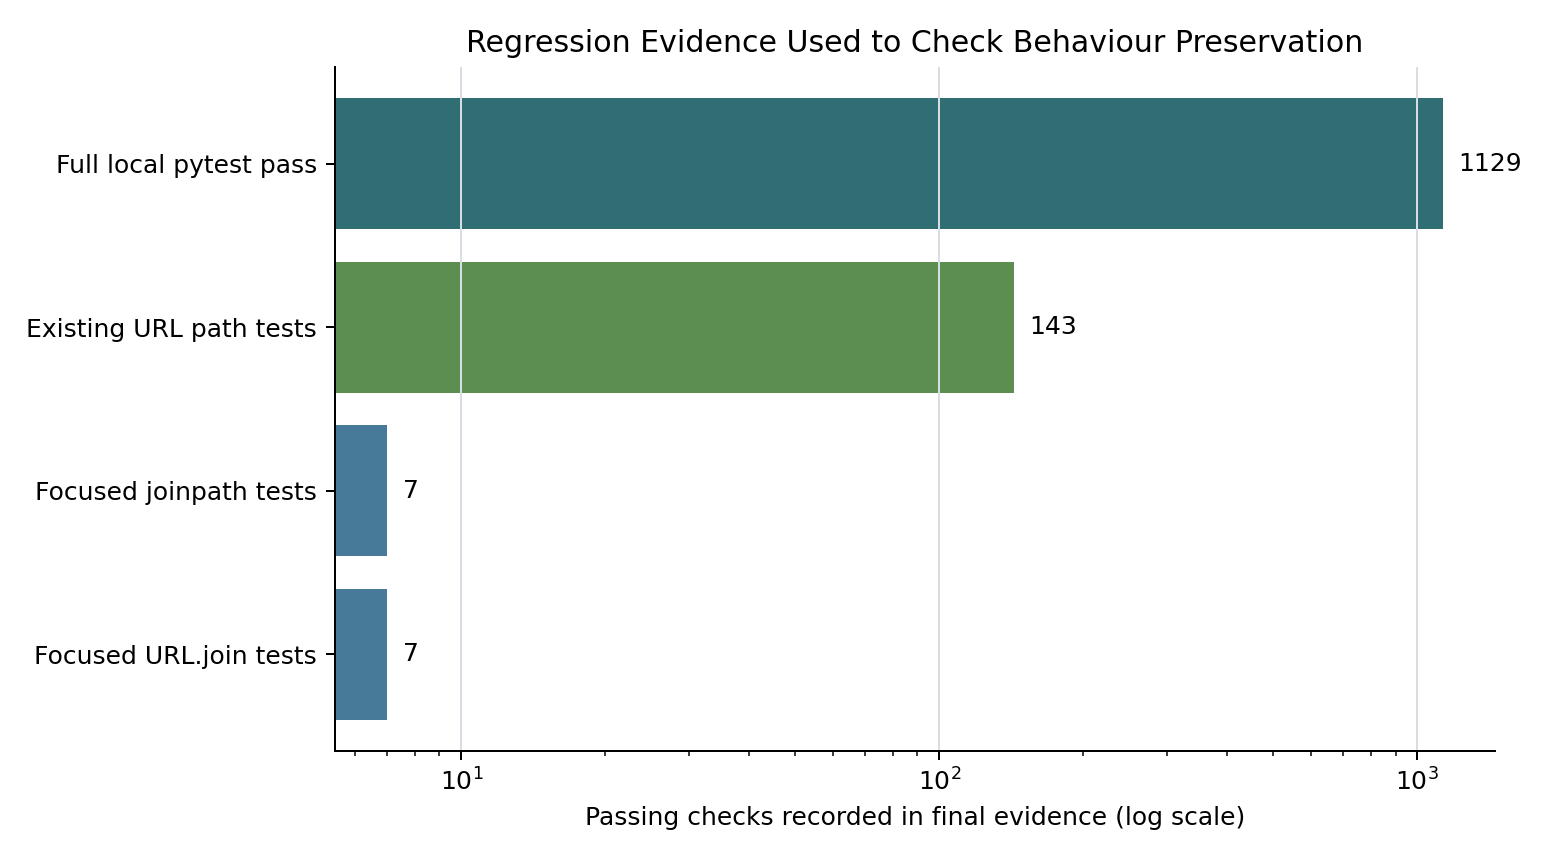
\includegraphics[width=0.82\textwidth]{assets/report_image_5.png}

\end{figure}

\begin{center}\small Figure 4. Regression evidence used to check behaviour preservation after restructuring.\end{center}

\subsection*{Risks and Limitations}


The main risk was behavioural regression in URL handling. This was mitigated by preserving the public API, adding focused tests before relying on the refactoring, running existing join-related tests, and running the full local suite. The project also avoided the highest-complexity URL.build() method because it would have required a broader test design and higher compatibility risk than the timeframe allowed.


The project focused on maintainability and modularity rather than performance. No benchmark result is claimed. The dynamic analysis is representative rather than exhaustive: it demonstrates runtime delegation for selected URL scenarios, but it does not prove all possible URL combinations. Finally, remote CI execution could not complete because of the GitHub account limitation, so the report relies on committed local verification outputs.


The main limitation is that the work does not claim a performance improvement. The dynamic analysis was used to understand runtime responsibility flow, not to benchmark speed. Another limitation is that the focused tests are representative rather than exhaustive. A production maintainer considering a larger URL-resolution rewrite would likely add broader specification-based or property-based tests. For this project, the selected scope was appropriate because it achieved the maintainability requirement without expanding the public API or adding unrequested functionality.


\section*{Conclusion}
\addcontentsline{toc}{section}{Conclusion}


\subsection*{Project Accomplishment}


The project completed a focused reengineering of a mature open-source library. The group first built an understanding of yarl through repository history, module inventory, public API inspection, baseline regression testing, coverage evidence, Radon complexity reports, and refactoring-commit mining. These techniques pointed to yarl/\_url.py as the central module and identified URL.join() and URL.\_make\_child() as achievable but meaningful targets.


The restructuring preserved the public API while moving detailed path-resolution responsibilities into more focused private helpers. URL.join() now delegates path, query, and fragment decisions to yarl/\_join.py. URL.\_make\_child() now delegates child path assembly to yarl/\_path.py. Together, these changes reduce the burden on yarl/\_url.py and make the relevant responsibilities easier to locate and test.


The final evidence shows that the work met its maintainability goals without breaking behaviour. The full local test suite passed with 1129 passed, 103 skipped, and 2 xfailed. The complexity of URL.join() improved from C (17) to B (8), and URL.\_make\_child() improved from C (17) to A (1). The new helper functions remained in acceptable complexity ranges, and dynamic traces confirmed that the new helper paths are exercised by representative URL operations.


\subsection*{Reflection}


The strongest part of the project was the controlled workflow: analyse first, add regression tests, make small refactorings, and then evaluate. This matched the needs of a library, where compatibility is more important than introducing visible new features. The decision not to refactor URL.build() was also important. Although it had the highest baseline complexity, it was broader and riskier, so choosing URL.join() and URL.\_make\_child() produced a more defensible result within the assignment timeframe.


The most challenging aspect was connecting different types of evidence into one coherent reengineering story. Static analysis alone could have led to a risky target, while tests alone would not explain why the target mattered. The final argument is stronger because repository history, static complexity, regression testing, and dynamic analysis all support the same conclusion: URL path-resolution responsibility was concentrated in \_url.py and could be safely decomposed.


With more time, the group would inspect URL.build() more deeply, add broader dynamic scenarios, and consider performance benchmarks for URL construction and joining. The group would also prefer a fully working remote CI run, but the account-level GitHub Actions limitation meant that local verification had to be recorded as the main evidence.


\subsection*{Member Reflections}


Dibing Bai: The most challenging part of the setup and baseline work was making the project evidence repeatable on a local machine. This was addressed by recording baseline outputs, keeping environment assumptions explicit, and using focused tests before relying on broader verification.


Yongjiang Liu: The most challenging part of coordination was turning separate analysis, testing, refactoring, GitHub, and report activities into one coherent reengineering argument. This was addressed by repeatedly checking the brief, keeping the target narrow, coordinating the branch and PR work, and linking report claims to committed evidence.


Jingxuan Wang: The most challenging part of static analysis was interpreting metrics without treating them as automatic decisions. This was addressed by combining Radon results with architecture review, code-smell reasoning, test adequacy, and risk assessment before choosing the final restructuring targets.


Ziqi Zhao: The most challenging part of regression testing was covering behaviour that users observe while the implementation details changed underneath. This was addressed by writing focused public-API tests for URL.join(), URL.joinpath(), and the / operator before accepting the helper extraction and path restructuring.


Xuhao Zhou: The most challenging part of evidence preparation was showing that the final result had been checked despite the GitHub Actions account limitation. This was addressed by restoring a minimal workflow, recording the remote failure reason, adding dynamic analysis evidence, and saving repeatable local verification outputs.


\section*{References}
\addcontentsline{toc}{section}{References}


\begin{longtable}{p{0.86\textwidth}}
\toprule
Reference \\
\midrule
aio-libs/yarl upstream repository: https://github.com/aio-libs/yarl \\
\addlinespace
Group repository: https://github.com/TUOS-COM-Reengineering-2026/group-project-pg\_05 \\
\addlinespace
Coursework base snapshot: e25e8d23e6912db52a23513ef1f6a17f889751ef \\
\addlinespace
pytest documentation: https://docs.pytest.org/ \\
\addlinespace
Radon documentation: https://radon.readthedocs.io/ \\
\addlinespace
PyDriller documentation: https://pydriller.readthedocs.io/ \\
\addlinespace
Python trace/profile tooling used through the standard library and project scripts in Submission/analysis. \\
\addlinespace
University of Sheffield brand toolkit: https://www.sheffield.ac.uk/brand-toolkit/introducing-our-brand-identity \\
\addlinespace
\bottomrule
\end{longtable}


\section*{Appendix A: AI Use Disclosure}
\addcontentsline{toc}{section}{Appendix A: AI Use Disclosure}


\subsection*{Acknowledge}


Generative AI tools, including ChatGPT and Codex, were used during this project as supporting tools. The project ideas, reengineering direction, target selection, technical judgements, and acceptance decisions came from the group members. AI tools were used to support wording, translation, code-editing assistance, and evidence organisation; they were not used as a replacement for group understanding, testing, or evaluation. Any AI-generated suggestions, wording, translation, or code-editing assistance were reviewed, checked against the repository evidence, and adapted by the group before being included in the report or repository.


\subsection*{Describe}


ChatGPT was used mainly to support communication, planning, translation, and report writing. It helped the group discuss possible workflows, interpret the coursework brief, organise the report structure, summarise testing and metric results, and turn group decisions into clearer English prose. Some group members drafted notes and explanations in Chinese and used AI-assisted translation or language polishing because they were less confident writing technical academic English directly. The translated or polished wording was then checked against the group's own understanding and the committed repository evidence.


Codex was used as a coding and repository assistant after the group had identified the reengineering direction and intended evidence chain. It helped apply small, reviewable code edits, prepare regression-test and analysis-support files, organise evidence under Submission/, inspect GitHub status, and update report wording to match the completed repository work. The group remained responsible for deciding which changes were appropriate, checking that public behaviour was preserved, running or reviewing the verification evidence, and deciding what to accept.


\subsection*{Evidence}


The evidence for the submitted work is in the repository rather than in the AI conversation. This includes the focused regression tests, yarl source changes, analysis scripts and outputs, local quality-check script, final pytest and Radon results, GitHub issues, pull requests, and commits listed in the following appendices. No source evidence, test result, commit record, or project decision is claimed solely on the basis of AI output. All accepted code changes were checked through focused regression tests, existing join-related tests, the full local test suite, and Radon complexity and maintainability checks.


\section*{Appendix B: Evidence Files}
\addcontentsline{toc}{section}{Appendix B: Evidence Files}


\begin{longtable}{p{0.43\textwidth} p{0.43\textwidth}}
\toprule
Evidence area & Repository evidence \\
\midrule
Baseline & Submission/baseline/baseline\_pytest.txt; python\_version.txt; pip\_freeze.txt; loc\_by\_file.csv; radon\_complexity.txt; radon\_maintainability.txt; coverage\_baseline.txt. \\
\addlinespace
System understanding & Submission/analysis/module\_inventory.csv; test\_inventory.csv; public\_api.txt; current\_system\_understanding.md. \\
\addlinespace
Evolution analysis & Submission/analysis/collect\_evolution\_metrics.py; commits\_by\_month.csv; loc\_over\_time.csv; refactoring\_commits.csv; evolution\_summary.md; reproducibility\_notes.md. \\
\addlinespace
Dynamic analysis & Submission/analysis/collect\_dynamic\_metrics.py; dynamic\_call\_counts.csv; dynamic\_module\_edges.csv; dynamic\_analysis\_summary.md. \\
\addlinespace
URL.join reengineering & tests/test\_url\_join\_regression.py; yarl/\_join.py; yarl/\_url.py; Submission/reengineering/before\_after\_url\_join\_refactor.md; url\_join\_module\_restructure\_summary.md. \\
\addlinespace
Child path reengineering & tests/test\_url\_joinpath\_regression.py; yarl/\_path.py; yarl/\_url.py; Submission/reengineering/url\_child\_path\_restructure\_summary.md. \\
\addlinespace
Final verification & Submission/final-check/code\_completion\_summary.md; final\_pytest\_result.txt; final\_radon\_complexity.txt; final\_radon\_maintainability.txt; local\_url\_join\_regression\_tests.txt; local\_url\_joinpath\_regression\_tests.txt; local\_existing\_join\_tests.txt; github\_actions\_status.md. \\
\addlinespace
\bottomrule
\end{longtable}


\section*{Appendix C: Selected Code Listings}
\addcontentsline{toc}{section}{Appendix C: Selected Code Listings}


\subsubsection*{Listing 1. Focused regression tests for URL.join()}


Path: tests/test\_url\_join\_regression.py


\begin{Verbatim}[breaklines=true,fontsize=\scriptsize]
1: from yarl import URL
   2: 
   3: import pytest
   4: 
   5: 
   6: @pytest.mark.parametrize(
   7:     ("base", "relative", "expected"),
   8:     [
   9:         (
  10:             "https://example.com/a/b/c",
  11:             "../d?x=1#frag",
  12:             "https://example.com/a/d?x=1#frag",
  13:         ),
  14:         (
  15:             "https://example.com/a/b/c",
  16:             "./d",
  17:             "https://example.com/a/b/d",
  18:         ),
  19:         (
  20:             "https://example.com/a/b/c",
  21:             "/root/path",
  22:             "https://example.com/root/path",
  23:         ),
  24:         (
  25:             "https://example.com/a/b/c?old=1#old-fragment",
  26:             "?new=2",
  27:             "https://example.com/a/b/c?new=2#old-fragment",
  28:         ),
  29:         (
  30:             "https://example.com/a/b/c?x=1",
  31:             "#section",
  32:             "https://example.com/a/b/c?x=1#section",
  33:         ),
  34:         (
  35:             "https://example.com/a/b/c",
  36:             "//cdn.example.com/lib.js",
  37:             "https://cdn.example.com/lib.js",
  38:         ),
  39:         (
  40:             "https://example.com/a/b/c",
  41:             "http://other.example.org/new",
  42:             "http://other.example.org/new",
  43:         ),
  44:     ],
  45: )
  46: def test_url_join_rfc3986_regression_cases(base, relative, expected):
  47:     result = URL(base).join(URL(relative))
  48: 
  49:     assert result == URL(expected)
\end{Verbatim}


\subsubsection*{Listing 2. Focused regression tests for URL.joinpath() and /}


Path: tests/test\_url\_joinpath\_regression.py


\begin{Verbatim}[breaklines=true,fontsize=\scriptsize]
1: from yarl import URL
   2: 
   3: import pytest
   4: 
   5: 
   6: @pytest.mark.parametrize(
   7:     ("base", "segments", "expected"),
   8:     [
   9:         (
  10:             "https://example.com",
  11:             ("alpha", "beta"),
  12:             "https://example.com/alpha/beta",
  13:         ),
  14:         (
  15:             "https://example.com/root/current?old=1#frag",
  16:             ("child",),
  17:             "https://example.com/root/current/child",
  18:         ),
  19:         (
  20:             "https://example.com/root/current/",
  21:             ("../sibling",),
  22:             "https://example.com/root/sibling",
  23:         ),
  24:         (
  25:             "https://example.com/root",
  26:             ("./child",),
  27:             "https://example.com/root/child",
  28:         ),
  29:         (
  30:             "relative/root",
  31:             ("../child",),
  32:             "relative/root/../child",
  33:         ),
  34:     ],
  35: )
  36: def test_joinpath_regression_path_assembly(
  37:     base: str, segments: tuple[str, ...], expected: str
  38: ) -> None:
  39:     assert str(URL(base).joinpath(*segments)) == expected
  40: 
  41: 
  42: def test_joinpath_regression_encoded_segment_preserves_raw_path() -> None:
  43:     joined = URL("https://example.com/base").joinpath("%2Fchild", encoded=True)
  44: 
  45:     assert joined.raw_path == "/base/%2Fchild"
  46: 
  47: 
  48: def test_truediv_regression_uses_joinpath_and_clears_query_fragment() -> None:
  49:     joined = URL("https://example.com/base?old=1#frag") / "child"
  50: 
  51:     assert str(joined) == "https://example.com/base/child"
\end{Verbatim}


\subsubsection*{Listing 3. Refactored URL.\_make\_child() and URL.join() excerpts}


Path: yarl/\_url.py


\begin{Verbatim}[breaklines=true,fontsize=\scriptsize]
1024:     def _make_child(self, paths: "Sequence[str]", encoded: bool = False) -> "URL":
1025:         netloc = self._netloc
1026:         path = _make_child_path(
1027:             self._path,
1028:             paths,
1029:             encoded=encoded,
1030:             has_netloc=bool(netloc),
1031:             path_quoter=PATH_QUOTER,
1032:         )
1033:         return from_parts(self._scheme, netloc, path, "", "")
   ...: ...
1387:     def join(self, url: "URL") -> "URL":
1388:         """Join URLs
1389: 
1390:         Construct a full ("absolute") URL by combining a "base URL"
1391:         (self) with another URL (url).
1392: 
1393:         Informally, this uses components of the base URL, in
1394:         particular the addressing scheme, the network location and
1395:         (part of) the path, to provide missing components in the
1396:         relative URL.
1397: 
1398:         """
1399:         if type(url) is not URL:
1400:             raise TypeError("url should be URL")
1401: 
1402:         scheme = url._scheme or self._scheme
1403:         if scheme != self._scheme or scheme not in USES_RELATIVE:
1404:             return url
1405: 
1406:         # scheme is in uses_authority as uses_authority is a superset of uses_relative
1407:         if (join_netloc := url._netloc) and scheme in USES_AUTHORITY:
1408:             return from_parts(scheme, join_netloc, url._path, url._query, url._fragment)
1409: 
1410:         join_path = url._path
1411:         path = _resolve_join_path(self, join_path) if join_path else self._path
1412: 
1413:         return from_parts(
1414:             scheme,
1415:             self._netloc,
1416:             path,
1417:             _resolve_join_query(self._query, join_path, url._query),
1418:             _resolve_join_fragment(self._fragment, join_path, url._fragment),
1419:         )
\end{Verbatim}


\subsubsection*{Listing 4. Private URL join helper module}


Path: yarl/\_join.py


\begin{Verbatim}[breaklines=true,fontsize=\scriptsize]
1: from typing import TYPE_CHECKING
   2: 
   3: from ._path import normalize_path
   4: 
   5: if TYPE_CHECKING:
   6:     from ._url import URL
   7: 
   8: 
   9: def _resolve_join_path(base: "URL", join_path: str) -> str:
  10:     orig_path = base._path
  11:     if join_path[0] == "/":
  12:         path = join_path
  13:     elif not orig_path:
  14:         path = f"/{join_path}"
  15:     elif orig_path[-1] == "/":
  16:         path = f"{orig_path}{join_path}"
  17:     else:
  18:         # ...
  19:         # and relativizing ".."
  20:         # parts[0] is / for absolute urls,
  21:         # this join will add a double slash there
  22:         path = "/".join([*base.parts[:-1], ""]) + join_path
  23:         # which has to be removed
  24:         if orig_path[0] == "/":
  25:             path = path[1:]
  26:     return normalize_path(path) if "." in path else path
  27: 
  28: 
  29: def _resolve_join_query(base_query: str, join_path: str, join_query: str) -> str:
  30:     return join_query if join_path or join_query else base_query
  31: 
  32: 
  33: def _resolve_join_fragment(
  34:     base_fragment: str, join_path: str, join_fragment: str
  35: ) -> str:
  36:     return join_fragment if join_path or join_fragment else base_fragment
\end{Verbatim}


\subsubsection*{Listing 5. Child path helper functions}


Path: yarl/\_path.py


\begin{Verbatim}[breaklines=true,fontsize=\scriptsize]
44: def _make_child_path(
  45:     base_path: str,
  46:     paths: Sequence[str],
  47:     *,
  48:     encoded: bool,
  49:     has_netloc: bool,
  50:     path_quoter: Callable[[str], str],
  51: ) -> str:
  52:     """
  53:     Add path elements to base_path, accounting for absolute vs relative paths.
  54: 
  55:     Existing empty segments are preserved, but new empty segments are not created.
  56:     """
  57:     parsed, needs_normalize = _make_child_segments(
  58:         paths, encoded=encoded, path_quoter=path_quoter
  59:     )
  60:     _extend_with_base_path(parsed, base_path)
  61: 
  62:     # If the netloc is present, inject a leading slash when adding a path to an
  63:     # absolute URL where there was none before.
  64:     if has_netloc and parsed and parsed[-1] != "":
  65:         parsed.append("")
  66: 
  67:     parsed.reverse()
  68:     if not has_netloc or not needs_normalize:
  69:         return "/".join(parsed)
  70: 
  71:     path = "/".join(normalize_path_segments(parsed))
  72:     # If normalizing the path segments removed the leading slash, add it back.
  73:     return f"/{path}" if path and path[0] != "/" else path
  74: 
  75: 
  76: def _make_child_segments(
  77:     paths: Sequence[str],
  78:     *,
  79:     encoded: bool,
  80:     path_quoter: Callable[[str], str],
  81: ) -> tuple[list[str], bool]:
  82:     parsed: list[str] = []
  83:     needs_normalize = False
  84:     for idx, path in enumerate(reversed(paths)):
  85:         # Empty segment of last is not removed.
  86:         last = idx == 0
  87:         if path and path[0] == "/":
  88:             raise ValueError(f"Appending path {path!r} starting from slash is forbidden")
  89: 
  90:         # The existing path is already quoted, so quote each new element before
  91:         # combining the old and new segments.
  92:         path = path if encoded else path_quoter(path)
  93:         needs_normalize |= "." in path
  94:         _extend_with_child_segments(parsed, path, last=last)
  95: 
  96:     return parsed, needs_normalize
  97: 
  98: 
  99: def _extend_with_child_segments(parsed: list[str], path: str, *, last: bool) -> None:
 100:     segments = path.split("/")
 101:     segments.reverse()
 102:     # Remove trailing empty segment for all but the last path.
 103:     parsed += segments[1:] if not last and segments[0] == "" else segments
 104: 
 105: 
 106: def _extend_with_base_path(parsed: list[str], base_path: str) -> None:
 107:     if not base_path:
 108:         return
 109: 
 110:     # If the old path ends with a slash, the last segment is an empty string
 111:     # and should be removed before adding the new path segments.
 112:     old_segments = base_path.split("/")
 113:     old = old_segments[:-1] if old_segments[-1] == "" else old_segments
 114:     old.reverse()
 115:     parsed += old
\end{Verbatim}


\subsubsection*{Listing 6. Local quality-check script}


Path: tools/run\_local\_checks.py


\begin{Verbatim}[breaklines=true,fontsize=\scriptsize]
34: def main() -> None:
  35:     OUT_DIR.mkdir(parents=True, exist_ok=True)
  36:     os.environ.setdefault("YARL_NO_EXTENSIONS", "1")
  37: 
  38:     run(
  39:         [sys.executable, "-m", "pytest", "-q", "--no-cov", "tests/test_url_join_regression.py"],
  40:         OUT_DIR / "local_url_join_regression_tests.txt",
  41:     )
  42: 
  43:     run(
  44:         [sys.executable, "-m", "pytest", "-q", "--no-cov", "tests/test_url_joinpath_regression.py"],
  45:         OUT_DIR / "local_url_joinpath_regression_tests.txt",
  46:     )
  47: 
  48:     run(
  49:         [
  50:             sys.executable,
  51:             "-m",
  52:             "pytest",
  53:             "-q",
  54:             "--no-cov",
  55:             "tests/test_url.py",
  56:             "-k",
  57:             "join or joinpath or div",
  58:         ],
  59:         OUT_DIR / "local_existing_join_tests.txt",
  60:     )
  61: 
  62:     run(
  63:         [sys.executable, "-m", "pytest", "-q", "--no-cov", "tests"],
  64:         OUT_DIR / "local_full_pytest.txt",
  65:         OUT_DIR / "final_pytest_result.txt",
  66:     )
  67: 
  68:     run(
  69:         [sys.executable, "-m", "radon", "cc", "yarl", "-s", "-a"],
  70:         OUT_DIR / "local_radon_complexity.txt",
  71:         OUT_DIR / "final_radon_complexity.txt",
  72:     )
  73: 
  74:     run(
  75:         [sys.executable, "-m", "radon", "mi", "yarl", "-s"],
  76:         OUT_DIR / "local_radon_maintainability.txt",
  77:         OUT_DIR / "final_radon_maintainability.txt",
  78:     )
  79: 
  80:     print("\nLocal quality checks completed successfully.")
  81: 
  82: 
  83: if __name__ == "__main__":
  84:     main()
\end{Verbatim}


\section*{Appendix D: GitHub Project Evidence}
\addcontentsline{toc}{section}{Appendix D: GitHub Project Evidence}


The repository history shows fine-grained commits, issues, and pull requests rather than one large final commit. The main merged pull requests were:


\begin{longtable}{p{0.29\textwidth} p{0.29\textwidth} p{0.29\textwidth}}
\toprule
PR & Title & Merged \\
\midrule
\#1 & Add system understanding and evolution analysis & 2026-05-13 \\
\addlinespace
\#2 & Refactor URL.join path resolution & 2026-05-16 \\
\addlinespace
\#3 & Evaluate URL.join refactoring impact & 2026-05-16 \\
\addlinespace
\#4 & Move URL.join helpers into private module & 2026-05-16 \\
\addlinespace
\#5 & Add local quality check script & 2026-05-16 \\
\addlinespace
\bottomrule
\end{longtable}


The main GitHub issues used to organise work were:


\begin{longtable}{p{0.29\textwidth} p{0.29\textwidth} p{0.29\textwidth}}
\toprule
Issue & Title & Status \\
\midrule
\#6 & Baseline setup and local regression testing & Closed \\
\addlinespace
\#7 & System understanding and baseline metrics & Closed \\
\addlinespace
\#8 & Upstream evolution analysis & Closed \\
\addlinespace
\#9 & Identify URL.join as reengineering target & Closed \\
\addlinespace
\#10 & Add URL.join regression tests & Closed \\
\addlinespace
\#11 & Refactor URL.join and evaluate impact & Closed \\
\addlinespace
\#12 & Add local quality-check script due to Actions quota & Closed \\
\addlinespace
\#13 & Prepare final report & Open during report preparation \\
\addlinespace
\bottomrule
\end{longtable}


Additional direct commits completed the final evidence chain after the earlier pull requests: 64cee18 Add URL.joinpath regression tests; eb405b9 Move child path assembly into path helpers; 26270ef Make analysis scripts reproducible; 309e713 Add dynamic analysis evidence for URL path operations; f5907a7 Restore minimal regression workflow triggers; 822f061 Refresh final verification evidence; c6f57ff Record GitHub Actions billing limitation. Later documentation commits on codex/update-final-report updated the final report and deliverables: c14989e Update final report with completed reengineering evidence; 2a71a9a Clarify AI use disclosure in final report; 5fa0ff0 Update report members and AI disclosure; 0529b57 Expand final report body and evidence figures. The code reengineering commits are the implementation commits listed before these documentation-only updates.


\section*{Appendix E: GitHub Actions Limitation}
\addcontentsline{toc}{section}{Appendix E: GitHub Actions Limitation}


A minimal GitHub Actions workflow was restored for regression testing. It supports manual execution and triggers on push or pull request changes affecting yarl source files, tests, or the workflow file. It uses ubuntu-24.04 and runs only the focused URL regression set plus existing join/joinpath/div tests, which follows the coursework guidance to use Actions only for essential checks.


The latest checked remote run was the Regression tests workflow on push to main at commit 822f0615793352dfa15179102c1eee4d8168c6ad. GitHub marked the run as completed with conclusion failure, but the check annotation stated that the job was not started because recent account payments had failed or the spending limit needed to be increased. No runner was allocated. This was therefore an account/billing limitation, not a failing test result from the project code.


Following the course guidance and to make validation repeatable, the group used local verification as the main evidence. tools/run\_local\_checks.py runs focused URL.join tests, focused URL.joinpath tests, existing URL join/joinpath/div tests, the full local pytest suite, Radon complexity, and Radon maintainability. The outputs are committed under Submission/final-check.


\end{document}
